\documentclass[12pt]{article}
\usepackage[utf8]{inputenc}
\usepackage{float}
\usepackage{amsmath}
\usepackage{tikz}

\usepackage[hmargin=3cm,vmargin=6.0cm]{geometry}
%\topmargin=0cm
\topmargin=-2cm
\addtolength{\textheight}{6.5cm}
\addtolength{\textwidth}{2.0cm}
%\setlength{\leftmargin}{-5cm}
\setlength{\oddsidemargin}{0.0cm}
\setlength{\evensidemargin}{0.0cm}

%misc libraries goes here



\begin{document}

\section*{Student Information } 
%Write your full name and id number between the colon and newline
%Put one empty space character after colon and before newline
Full Name : Batuhan Karaca \\
Id Number : 2310191 \\

% Write your answers below the section tags
\section*{Answer 1}
\textbf{a)}Let us observe the number of bit strings with length of $n$ such that there will not come $1$ 
immediately after every bit $1$(this is \textit{rule 1}), called $g_n$. Assume, every distinct 
ordering of bits of length $n$ abiding by \textit{rule 1} is accumulated in a set $S$.
Two disjoint subsets of $S$ for cases, can be considered, strings starting with $1$ or $0$
\\ \\
\begin{tabular}{l}
    $A=\{c\ |\ c=0\ \_\ \_\ \_\ \_\ ...\_\ \_\ \_\ \_\ \} $\\
    $B=\{c\ |\ c=1\ 0\ \_\ \_\ \_\ ...\_\ \_\ \_\ \_\ \} $\\
    $S=A\cup B$\\
\end{tabular}
\\ \\
$\_$ is for unknown bits.
If the first bit is $0$, we don't know about the remaining bits but else, the second bit must be $0$ by \textit{rule 1}.
Since both cases are disjoint subsets, we can use the sum rule such that $|S|=|A|+|B|$.
Both $A$, $B$ should abide by the rule of their super set $S$ which is \textit{rule 1}. Since there remains no such 
limitation against \textit{rule 1} in both subsets, 
the set $A$ is with unknown $n-1$ bits has cardinality $g_{n-1}$; similarly set $B$, $g_{n-2}$.
Hence, the number of bit strings with length of $n$, $g_n=|S|$
\\ \\
\begin{tabular}{l}
    $g_n=g_{n-1} + g_{n-2}$\\
    $g_1=2$ and $g_2=3$ by counting manually\\
    $g_0=g_2-g_1=1$\\
\end{tabular} 
\\ \\
We solve the recurrence relation. Characteristic equation is $r^2-r-1=0$ with $r=\frac{1\pm \sqrt{5}}{2}$
\\ \\
\begin{tabular}{l}
    $g_n=\alpha_1r_1^n+\alpha_2r_2^n$\\
    $g_n=\alpha_1(\frac{1+ \sqrt{5}}{2})^n+\alpha_2(\frac{1- \sqrt{5}}{2})^n$\\
    $g_0=\alpha_1+\alpha_2=1$\\
    $g_1=(\frac{1+ \sqrt{5}}{2})\alpha_1+(\frac{1- \sqrt{5}}{2})\alpha_2=2$\\
    $\alpha_1=\frac{5+ 3\sqrt{5}}{10}$\\
    $\alpha_2=\frac{5- 3\sqrt{5}}{10}$\\
    $g_n=(\frac{5+ 3\sqrt{5}}{10})(\frac{1+ \sqrt{5}}{2})^n+(\frac{5- 3\sqrt{5}}{10})(\frac{1- \sqrt{5}}{2})^n$\\
\end{tabular} 
\\ \\
We have, of the question another rule, \textit{rule 2} that is every bit $1$ must be followed immediately by a bit $0$.
The number of such bit strings of length of $n$ is $f_n$. 
Then, there is an additional case to \textit{rule 1} that there exist no $1$ at the end.
Similarly, we form another set complying with \textit{rule 2}, $S_0$ with two subsets
\\ \\
\begin{tabular}{l}
    $A_0=\{c\ |\ c=0\ \_\ \_\ \_\ \_\ ...\_\ \_\ \_\ 0\ \} $\\
    $B_0=\{c\ |\ c=1\ 0\ \_\ \_\ \_\ ...\_\ \_\ \_\ 0\ \} $\\
    $S_0=A_0\cup B_0$\\
\end{tabular}
\\ \\
Last bits are $0$ because of \textit{rule 2} since there is a limitation of no $1$s at the end.
The last unknown bit can be any bit as long as it complies with \textit{rule 1}.
Then, $A_0$ has the cardinality of $g_{n-2}$, likewise $B_0$ $g_{n-3}$. Similarly since subsets are 
disjoint, by the sum rule
\\ \\
\begin{tabular}{l}
    $f_n=g_{n-2} + g_{n-3}$\\
    $f_n=g_{n-1}$\\
    $f_n=(\frac{5+ 3\sqrt{5}}{10})(\frac{1+ \sqrt{5}}{2})^{n-1}+(\frac{5- 3\sqrt{5}}{10})(\frac{1- \sqrt{5}}{2})^{n-1}$\\
    $f_9=55$\\
\end{tabular}
\\ \\
\textbf{NOTE:} Since the case that the string is made up of all zeros is excluded, the answer is
$55-1=54$.
\\ \\ \\ \\
\textbf{b)}By the request that the question gives, we understand there are at least $8$ $1$s 
in a bit string of length $10$. Then there are three distinct cases
\\ \\
\begin{tabular}{l}
    $8\ 1s$ and $2\ 0s \quad (case 1)$\\
    $9\ 1s$ and a single $0 \quad (case 2)$\\
    $10\ 1s \quad (case 3)$\\
\end{tabular}
\\ \\
We have a list of orderings, which can be solved by using permutations, however there are repeating
values $0$ and $1$. Then we use
\\ \\
\begin{tabular}{l}
    $\frac{n!}{r_1!r_2!...r_k!}$\\
\end{tabular}
\\ \\
for ordering $n$ items which have $k$ repetitive values with multiplicity $r_i$. In our cases,
\\ \\
\begin{tabular}{l}
    $\frac{10!}{8!2!}=45$ for $(case 1)$\\
    \\
    $\frac{10!}{9!1!}=10$ for $(case 2)$\\
    \\
    $\frac{10!}{10!}=1$ for $(case 1)$\\
    \\
\end{tabular}
\\ \\
Since the cases are distinct, by the sum rule we can add them to achieve the total number, 
$45+10+1=56$
\\ \\ \\ \\
\textbf{c)}In the textbook (8th Edition) page 588
\\ \\
\begin{tabular}{l}
    \textit{Let $m$ and $n$ be positive integers with $m \geq n$. Then, there are}\\ \\
    \textit{$\quad n^m-C(n,1)(n-1)^m+C(n,2)(n-2)^m\ ...\ +(-1)^{n-1}C(n,n-1)(1)^m $}\\ \\
    \textit{onto functions from a set with m elements to a set with n elements.}\\
\end{tabular}
\\ \\
Then, in this case $m=4$ and $n=3$, and the number of onto functions
\\ \\
\begin{tabular}{l}
    $3^4-C(3,1)2^4+C(3,2)1^4=81-(3*16)+3=36$\\
\end{tabular}
\\ \\ \\ \\
\textbf{d)}We will use abbreviations for lectures, $D$ and $S$ respectively. We have a
table of different cases -integers indicate the number of items chosen.
\\ \\
\begin{tabular}{|l|l|l}
    \cline{1-2}
    $D$ & $S$ & \\
    \cline{1-2}
    $1$ & $3$ & $(case 1)$\\
    \cline{1-2}
    $2$ & $2$ & $(case 2)$\\
    \cline{1-2}
    $3$ & $1$ & $(case 3)$\\
    \cline{1-2}
\end{tabular}
\\ \\ \\ \\
\textbf{\textit{1)if the books are \emph{IDENTICAL} in their respective groups}}
\\ \\
If the books are identical, observing each case seperately, not only the order we choose does not matter, 
but also which book we choose does not matter. Why the order does not matter is because, we choose from 
a set, we form a subset. This is common to the second case, in which the books are distinct -detailed 
explanation is given in that second section, with the definiton of r-combination. Secondly, which book
we choose does not matter. For instance we choose a $D$ book, $3$ $S$ books. The other $4$ $D$ books
were to be chosen, would not change the selection, since the same as the book we have chosen.
This is also the same for the $S$ books. Then, selections are the same. Hence, we have one selection 
for each case.
We have $1+1+1=3$ selections.
\\ \\
\textbf{\textit{2)if the books are \emph{DISTINCT} in their respective groups}}
\\ \\
Each case can be broken down to two sequence
of tasks, firstly choosing a $D$ book and then choosing a $S$ book or vice versa. Both orders 
give the same number of decisions, then this aspect satisfies the commutative principle. We can use
product rule to find the number of decisions for each case seperately, by lining numbers of choices
and multiply.  
In the textbook (8th Edition) page 431
\\ \\
\begin{tabular}{l}
    \textit{An r-combination of elements of a set is an unordered selection of r elements from the set.Thus,}\\
    \textit{an r-combination is simply a subset of the set with r elements.}\\
\end{tabular}
\\ \\
Since we choose books from the list, changing the order in the list of chosen books is the same.
Then we work with unordered sets here, than we are counting combinations of books. Hence for each case,
number of combinations, by utilizing product rule and combination.
\\ \\
\begin{tabular}{l}
    $C(item_1, chosen_1)*C(item_2, chosen_2)$\\
\end{tabular}
\\ \\
The cases are distinct, then we can use sum rule that we add up every number of combinations
each case offers to the total desired amount. Then, the total amount is
\\ \\
\begin{tabular}{l}
    $\sum\limits_{i=1}^n C(item_{1_i}, chosen_{1_i})*C(item_{2_i}, chosen_{2_i})$\\
\end{tabular}
\\ \\
$i$ to iterate all cases. $n=3$ in our case. For our case the result is
\\ \\
\begin{tabular}{l}
    $C(5,1)*C(7,3)+C(5,2)*C(7,2)+C(5,3)*C(7,1)=455$\\
\end{tabular}
\section*{Answer 2}
\textbf{a)}Observe a bit string of length $n$. We can set a relation between the bit string 
and the set $S=\{1,2,...,n\}$ such that $i$th element of the bit string is $1$ if 
$i$th element of the sequence $(1,2,...,n)$ is in the subset of $S$, $0$ otherwise.
Since every set containing exactly the same elements with different orders are equal(sets are
unordered), it is sufficient to only count the cases that no consecutive $1$s occur at the
string, without any additional calculation such as ordering. In other words, there is 
no $1$ immediately after every $1$, which is the same as \textit{rule 1} in \textbf{\textit{Answer 1 part a}}. 
Assume the count of strings is $g_n$. We can directly copy the result of \textit{rule 1}
\\ \\
\begin{tabular}{l}
    $g_n=g_{n-1} + g_{n-2}$\\
    $g_1=2$ and $g_2=3$ by counting manually\\
    $g_0=g_2-g_1=1$\\
\end{tabular} 
\\ \\ \\ \\
\textbf{b)}
\\ \\
\begin{tabular}{l}
    $f(x)=\sum_{i=0}^{\infty}g_ix^i \quad (1)$\\
    \\
    $xf(x)=\sum_{i=0}^{\infty}g_ix^{i+1}=\sum_{j=1}^{\infty}g_{i-1}x^i=\sum_{j=2}^{\infty}g_{i-1}x^i+g_0x$\\
    \\
    $x^2f(x)=\sum_{i=0}^{\infty}g_ix^{i+2}=\sum_{j=2}^{\infty}g_{i-2}x^i$\\
    \\
    $x^2f(x)+xf(x)=\sum_{i=2}^{\infty}g_{i-2}x^i+\sum_{j=2}^{\infty}g_{i-1}x^i+g_0x$\\
    \\
    $x^2f(x)+xf(x)=\sum_{i=2}^{\infty}g_ix^i+g_0x$\\
    \\
    $x^2f(x)+xf(x)=\sum_{i=0}^{\infty}g_ix^i-g_1x-g_0+g_0x$\\
    \\
    $x^2f(x)+xf(x)=\sum_{i=0}^{\infty}g_ix^i-2x-1+(1)x$\\
    \\
    $x^2f(x)+xf(x)=\sum_{i=0}^{\infty}g_ix^i-x-1$\\
    \\
    $(x^2+x)f(x)=f(x)-x-1$\\
    \\
    $f(x)=\frac{x+1}{1-x-x^2}$\\
    \\
\end{tabular} 
\\ \\
Since $\delta=b^2-4ac>0$, the equation $1-x-x^2=0$ has two unequal roots $r_1, r_2$ such that both 
are in the set $\{r\ |\ r=\frac{-1\pm \sqrt{5}}{2}  \}$.
\\ \\
\begin{tabular}{l}
    $f(x)=\frac{A}{r_1-x}+\frac{B}{x-r_2}=\frac{x+1}{1-x-x^2}$\\
\end{tabular}
\\ \\
Solving for $A, B$ gives $A=\frac{1+r_1}{r_1-r_2}$ and $B=\frac{1+r_2}{r_1-r_2}$. We wont expand 
for simplicity
\\ \\
\begin{tabular}{l}
    $f(x)=\frac{A}{r_1-x}+\frac{B}{x-r_2}$\\
    \\
    $f(x)=(\frac{A}{r_1})(\frac{1}{1-(x/r_1)})-(\frac{B}{r_2})(\frac{1}{1-(x/r_2)})$\\
\end{tabular}
\\ \\
We know $\frac{1}{1-(ax)}=\sum_{i=0}^{\infty}(ax)^i$
\\ \\
\begin{tabular}{l}
    $f(x)=(\frac{A}{r_1})(\sum_{i=0}^{\infty}(x/r_1)^i)-(\frac{B}{r_2})(\sum_{i=0}^{\infty}(x/r_2)^i)$\\
    \\
    $f(x)=\sum_{i=0}^{\infty}[A(\frac{1}{r_1})^{i+1}-B(\frac{1}{r_2})^{i+1}]x^i$\\
\end{tabular}
\\ \\
From the equation $(1)$
\\ \\
\begin{tabular}{l}
    $f(x)=\sum_{i=0}^{\infty}g_ix^i=\sum_{i=0}^{\infty}[A(\frac{1}{r_1})^{i+1}-B(\frac{1}{r_2})^{i+1}]x^i$\\
    \\
    $g_n=A(\frac{1}{r_1})^{n+1}-B(\frac{1}{r_2})^{n+1}$
\end{tabular}
\\ \\
Substituting $A, B, r_1, r_2$-(values $r1, r2$ are interchangeable)
\\ \\
\begin{tabular}{l}
    $g_n=\frac{1}{\sqrt{5}}((\frac{1+\sqrt{5}}{2})^{n+2}-(\frac{1-\sqrt{5}}{2})^{n+2})$
\end{tabular}
\section*{Answer 3}
Solving the characteristic equation
\\ \\
\begin{tabular}{l}
    $r^3-4r^2-r+4=0$\\
    $(r^2-1)(r-4)=0$\\
    $(r-1)(r+1)(r-4)=0$\\
    $r=\{ -1,1,4 \}$ is the set of characteristic roots\\
    \\
    $a_n=\alpha_1r_1^n+\alpha_2r_2^n+\alpha_3r_3^n$\\
    $a_n=\alpha_1(-1)^n+\alpha_2(1)^n+\alpha_3(4)^n$\\
    $a_n=\alpha_1(-1)^n+\alpha_2+\alpha_3(4)^n$\\
    \\
    $a_0=4$, $a_1=8$ and $a_2=34$\\
    \\
    $a_0=\alpha_1+\alpha_2+\alpha_3=4 \quad (1)$\\
    $a_1=-\alpha_1+\alpha_2+4\alpha_3=8 \quad (2)$\\
    $a_2=\alpha_1+\alpha_2+16\alpha_3=34 \quad (3)$\\
\end{tabular}
\\ \\
Solving $(1)$,$(2)$ and $(3)$ gives $\alpha_1=1$, $\alpha_2=1$ and $\alpha_3=2$. We have
\\ \\
\begin{tabular}{l}
    $a_n=(1)(-1)^n+(1)+(2)(4)^n$\\
    $a_n=2(4)^n+(-1)^n+1$\\
\end{tabular}
\section*{Answer 4}
By definition, in order that $R$ is an equivalence equation, $R$ should be 
\textit{reflexive, symmetric,} and \textit{transitive}. 
\\ \\
\textit{\textbf{1)Is R reflexive?}}
\\ \\
For any real numbers $r_1,\ r_2$
\\ \\
\begin{tabular}{l}
    $3r_1-2r_2=3r_1-2r_2$\\
\end{tabular}
\\ \\
Then $(r_1,r_2)R(r_1,r_2)$, hence $R$ is reflexive
\\ \\
\textit{\textbf{1)Is R symmetric?}}
\\ \\
For any real numbers $r_1,\ r_2,\ r_3,\ r_4$ assume $(r_1,r_2)R(r_3,r_4)$. Then
\\ \\
\begin{tabular}{l}
    $3r_1-2r_2=3r_3-2r_4$\\
\end{tabular}
\\ \\
If $3r_1-2r_2=3r_3-2r_4$, $3r_3-2r_4=3r_1-2r_2$ is also true. Then
$(r_3,r_4)R(r_1,r_2)$, hence $R$ is symmetric.
\\ \\
\textit{\textbf{1)Is R transitive?}}
\\ \\
For any real numbers $r_1,\ r_2,\ r_3,\ r_4,\ r_5,\ r_6$ assume 
$(r_1,r_2)R(r_3,r_4)\ (1)$ and $(r_3,r_4)R(r_5,r_6)\ (2)$. Then
\\ \\
\begin{tabular}{l l l}
    $3r_1-2r_2=3r_3-2r_4$ & & (by the relation $(1)$)\\
    $3r_3-2r_4=3r_5-2r_6$ & & (by the relation $(2)$)\\
\end{tabular}
\\ \\
by the above equations,
\\ \\
\begin{tabular}{l}
    $3r_1-2r_2=3r_5-2r_6$\\
\end{tabular}
\\ \\
Then $(r_1,r_2)R(r_5,r_6)$, hence $R$ is transitive.
\\ \\ \\ \\
By definition, the equivalence class of $a$ is a set $[a]_R=\{s\ |\ aRs\ \}$. Then, 
the equivalence class of $(2,3)$ is
\\ \\
\begin{tabular}{l}
    $[(2,3)]_R=\{(x,y)\ |\ (2,3)R(x,y)\ \}$\\
    $[(2,3)]_R=\{(x,y)\ |\ 3(2)-2(3)=3x-2y\ \}$\\
    $[(2,3)]_R=\{(x,y)\ |\ 3x-2y=0\ \}$\\
\end{tabular}
\\ \\
Similarly, the equivalence class of $(2,-3)$ is
\\ \\
\begin{tabular}{l}
    $[(2,-3)]_R=\{(x,y)\ |\ (2,-3)R(x,y)\ \}$\\
    $[(2,-3)]_R=\{(x,y)\ |\ 3(2)-2(-3)=3x-2y\ \}$\\
    $[(2,-3)]_R=\{(x,y)\ |\ 3x-2y=12\ \}$\\
\end{tabular}
\\ \\
Graphical representations of $[(2,3)]$ and $[(2,-3)]$
\\ \\
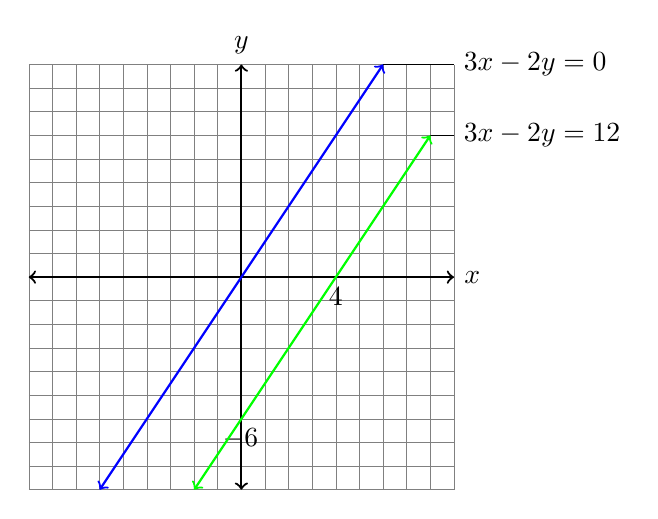
\begin{tikzpicture}[scale=0.3]
    %grid
    \draw[step=1cm,gray,very thin] (-9,-9) grid (9,9);
    %numbers and graphs
    \draw (4 cm,1pt) -- (4 cm,-1pt) node[anchor=north] {$4$};
    \draw (1pt,-6 cm) -- (-1pt,-6 cm) node[anchor=north] {$-6$};

    \draw[fill=none] (6,9) -- (9,9) node[anchor=west] {$3x-2y=0$};
    \draw[fill=none] (8,6) -- (9,6) node[anchor=west] {$3x-2y=12$};

    %axes
    \draw[thick,->] (0,0) -- (9,0) node[anchor=west] {$x$};
    \draw[thick,->] (0,0) -- (-9,0);
    \draw[thick,->] (0,0) -- (0,9) node[anchor=south] {$y$};
    \draw[thick,->] (0,0) -- (0,-9);

    %plot lines
    \draw[thick,->,blue] (0,0) -- (6,9);
    \draw[thick,->,blue] (0,0) -- (-6,-9);
    
    \draw[thick,->,green] (2,-3) -- (8,6);
    \draw[thick,->,green] (2,-3) -- (-2,-9);
\end{tikzpicture}
\end{document}
